\documentclass[../main/NEMO_manual]{subfiles}

\begin{document}

\chapter{A brief guide to the DOMAINcfg tool}
\label{apdx:DOMCFG}

%    {\em 4.0} & {\em Andrew Coward} & {\em Created at v4.0 from materials removed from chap\_DOM that are still relevant to the \forcode{DOMAINcfg} tool and which illustrate and explain the choices to be made by the user when setting up new domains }  \\

\thispagestyle{plain}

\chaptertoc

\paragraph{Changes record} ~\\

{\footnotesize
  \begin{tabularx}{\textwidth}{l||X|X}
    Release & Author(s) & Modifications \\
    \hline
    {\em   4.0} & {\em ...} & {\em ...} \\
    {\em   3.6} & {\em ...} & {\em ...} \\
    {\em   3.4} & {\em ...} & {\em ...} \\
    {\em <=3.4} & {\em ...} & {\em ...}
  \end{tabularx}
}

\clearpage

This appendix briefly describes some of the options available in the
\forcode{DOMAINcfg} tool mentioned in \autoref{chap:DOM}.

This tool will evolve into an independent utility with its own documentation but its
current manifestation is mostly a wrapper for \NEMO\ \forcode{DOM} modules more aligned to
those in the previous versions of \NEMO. These versions allowed the user to define some
horizontal and vertical grids through additional namelist parameters. Explanations of
these parameters are retained here for reference pending better documentation for
\forcode{DOMAINcfg}. Please note that the namelist blocks named in this appendix refer to
those read by \forcode{DOMAINcfg} via its own \forcode{namelist_ref} and
\forcode{namelist_cfg} files. Although, due to their origins, these namelists share names
with those used by \NEMO, they are not interchangeable and should be considered independent
of those described elsewhere in this manual.

%% =================================================================================================
\section{Choice of horizontal grid}
\label{sec:DOMCFG_hor}

\begin{listing}
  \nlst{namdom_domcfg}
  \caption{\forcode{&namdom_domcfg}}
  \label{lst:namdom_domcfg}
\end{listing}

The user has three options available in defining a horizontal grid, which involve the
namelist variable \np{jphgr_mesh}{jphgr\_mesh} of the \nam{dom}{dom} (\texttt{DOMAINcfg} variant only)
namelist.

\begin{description}
 \item [{\np{jphgr_mesh}{jphgr\_mesh}=0}]  The most general curvilinear orthogonal grids.
  The coordinates and their first derivatives with respect to $i$ and $j$ are provided
  in a input file (\ifile{coordinates}), read in \rou{hgr\_read} subroutine of the domhgr module.
  This is now the only option available within \NEMO\ itself from v4.0 onwards.
\item [{\np{jphgr_mesh}{jphgr\_mesh}=1 to 5}] A few simple analytical grids are provided (see below).
  For other analytical grids, the \mdl{domhgr} module (\texttt{DOMAINcfg} variant) must be
  modified by the user. In most cases, modifying the \mdl{usrdef\_hgr} module of \NEMO\ is
  a better alternative since this is designed to allow simple analytical domains to be
  configured and used without the need for external data files.
\end{description}

There are two simple cases of geographical grids on the sphere. With
\np{jphgr_mesh}{jphgr\_mesh}=1, the grid (expressed in degrees) is regular in space,
with grid sizes specified by parameters \np{ppe1_deg}{ppe1\_deg} and \np{ppe2_deg}{ppe2\_deg},
respectively. Such a geographical grid can be very anisotropic at high latitudes
because of the convergence of meridians (the zonal scale factors $e_1$
become much smaller than the meridional scale factors $e_2$). The Mercator
grid (\np{jphgr_mesh}{jphgr\_mesh}=4) avoids this anisotropy by refining the meridional scale
factors in the same way as the zonal ones. In this case, meridional scale factors
and latitudes are calculated analytically using the formulae appropriate for
a Mercator projection, based on \np{ppe1_deg}{ppe1\_deg} which is a reference grid spacing
at the equator (this applies even when the geographical equator is situated outside
the model domain).

In these two cases (\np{jphgr_mesh}{jphgr\_mesh}=1 or 4), the grid position is defined by the
longitude and latitude of the south-westernmost point (\np{ppglamt0}
and \np{ppgphi0}{ppgphi0}). Note that for the Mercator grid the user need only provide
an approximate starting latitude: the real latitude will be recalculated analytically,
in order to ensure that the equator corresponds to line passing through $t$-
and $u$-points.

Rectangular grids ignoring the spherical geometry are defined with
\np{jphgr_mesh}{jphgr\_mesh} = 2, 3, 5. The domain is either an $f$-plane (\np{jphgr_mesh}{jphgr\_mesh} = 2,
Coriolis factor is constant) or a beta-plane (\np{jphgr_mesh}{jphgr\_mesh} = 3, the Coriolis factor
is linear in the $j$-direction). The grid size is uniform in meter in each direction,
and given by the parameters \np{ppe1_m}{ppe1\_m} and \np{ppe2_m}{ppe2\_m} respectively.
The zonal grid coordinate (\textit{glam} arrays) is in kilometers, starting at zero
with the first $t$-point. The meridional coordinate (gphi. arrays) is in kilometers,
and the second $t$-point corresponds to coordinate $gphit=0$. The input
variable \np{ppglam0}{ppglam0} is ignored. \np{ppgphi0}{ppgphi0} is used to set the reference
latitude for computation of the Coriolis parameter. In the case of the beta plane,
\np{ppgphi0}{ppgphi0} corresponds to the center of the domain. Finally, the special case
\np{jphgr_mesh}{jphgr\_mesh}=5 corresponds to a beta plane in a rotated domain for the
GYRE configuration, representing a classical mid-latitude double gyre system.
The rotation allows us to maximize the jet length relative to the gyre areas
(and the number of grid points).

%% =================================================================================================
\section{Vertical grid}
\label{sec:DOMCFG_vert}

%% =================================================================================================
\subsection{Vertical reference coordinate}
\label{sec:DOMCFG_zref}

\begin{figure}[!tb]
  \centering
  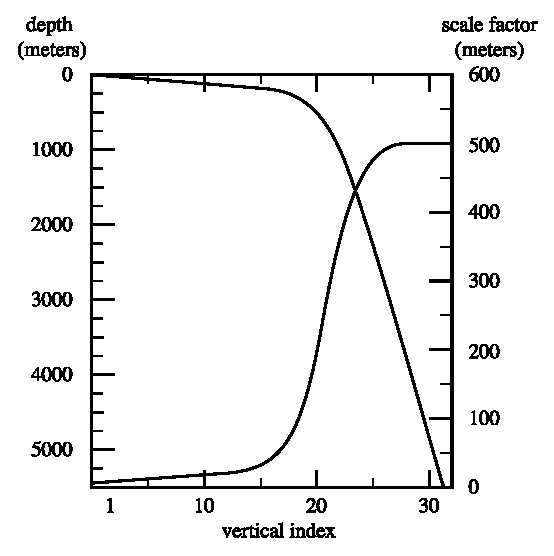
\includegraphics[width=0.66\textwidth]{DOMCFG_zgr}
  \caption[DOMAINcfg: default vertical mesh for ORCA2]{
    Default vertical mesh for ORCA2: 30 ocean levels (L30).
    Vertical level functions for (a) T-point depth and (b) the associated scale factor for
    the $z$-coordinate case.}
  \label{fig:DOMCFG_zgr}
\end{figure}

The reference coordinate transformation $z_0(k)$ defines the arrays $gdept_0$ and
$gdepw_0$ for $t$- and $w$-points, respectively. See \autoref{sec:DOMCFG_sco} for the
S-coordinate options.  As indicated on \autoref{fig:DOM_index_vert} \jp{jpk} is the number of
$w$-levels.  $gdepw_0(1)$ is the ocean surface.  There are at most \jp{jpk}-1 $t$-points
inside the ocean, the additional $t$-point at $jk = jpk$ is below the sea floor and is not
used.  The vertical location of $w$- and $t$-levels is defined from the analytic
expression of the depth $z_0(k)$ whose analytical derivative with respect to $k$ provides
the vertical scale factors.  The user must provide the analytical expression of both $z_0$
and its first derivative with respect to $k$.  This is done in routine \mdl{domzgr}
through statement functions, using parameters provided in the \nam{dom}{dom} namelist
(\texttt{DOMAINcfg} variant).

It is possible to define a simple regular vertical grid by giving zero stretching
(\np[=0]{ppacr}{ppacr}).  In that case, the parameters \jp{jpk} (number of $w$-levels)
and \np{pphmax}{pphmax} (total ocean depth in meters) fully define the grid.

For climate-related studies it is often desirable to concentrate the vertical resolution
near the ocean surface.  The following function is proposed as a standard for a
$z$-coordinate (with either full or partial steps):
\begin{gather}
  \label{eq:DOMCFG_zgr_ana_1}
    z_0  (k) = h_{sur} - h_0 \; k - \; h_1 \; \log  \big[ \cosh ((k - h_{th}) / h_{cr}) \big] \\
    e_3^0(k) = \lt|    - h_0      -    h_1 \; \tanh \big[        (k - h_{th}) / h_{cr}  \big] \rt|
\end{gather}

where $k = 1$ to \jp{jpk} for $w$-levels and $k = 1$ to $k = 1$ for $t-$levels.  Such an
expression allows us to define a nearly uniform vertical location of levels at the ocean
top and bottom with a smooth hyperbolic tangent transition in between (\autoref{fig:DOMCFG_zgr}).

A double hyperbolic tangent version (\np[=.true.]{ldbletanh}{ldbletanh}) is also available
which permits finer control and is used, typically, to obtain a well resolved upper ocean
without compromising on resolution at depth using a moderate number of levels.

\begin{gather}
  \label{eq:DOMCFG_zgr_ana_1b}
    \begin{split}
    z_0  (k) = h_{sur} - h_0 \; k &- \; h_1 \; \log  \big[ \cosh ((k - h_{th}) / h_{cr}) \big] \\
                             \;   &- \; h2_1 \; \log  \big[ \cosh ((k - h2_{th}) / h2_{cr}) \big]
    \end{split}
\end{gather}
\begin{gather}
    \begin{split}
    e_3^0(k) = \big|    - h_0    &-   h_1 \; \tanh \big[       (k - h_{th})  / h_{cr}   \big]  \\
                                 &-  h2_1 \; \tanh \big[       (k - h2_{th}) / h2_{cr}  \big] \big|
    \end{split}
\end{gather}

If the ice shelf cavities are opened (\np[=.true.]{ln_isfcav}{ln\_isfcav}), the definition
of $z_0$ is the same.  However, definition of $e_3^0$ at $t$- and $w$-points is
respectively changed to:
\begin{equation}
  \label{eq:DOMCFG_zgr_ana_2}
  \begin{split}
    e_3^T(k) &= z_W (k + 1) - z_W (k    ) \\
    e_3^W(k) &= z_T (k    ) - z_T (k - 1)
  \end{split}
\end{equation}

This formulation decreases the self-generated circulation into the ice shelf cavity
(which can, in extreme case, leads to numerical instability). This is now the recommended formulation for all configurations using v4.0 onwards. The analytical derivation of thicknesses is maintained for backwards compatibility.

The most used vertical grid for ORCA2 has $10~m$ ($500~m$) resolution in the surface
(bottom) layers and a depth which varies from 0 at the sea surface to a minimum of
$-5000~m$.  This leads to the following conditions:

\begin{equation}
  \label{eq:DOMCFG_zgr_coef}
  \begin{array}{ll}
    e_3 (1   + 1/2) =  10. & z(1  ) =     0. \\
    e_3 (jpk - 1/2) = 500. & z(jpk) = -5000.
  \end{array}
\end{equation}

With the choice of the stretching $h_{cr} = 3$ and the number of levels \jp{jpk}~$= 31$,
the four coefficients $h_{sur}$, $h_0$, $h_1$, and $h_{th}$ in
\autoref{eq:DOMCFG_zgr_ana_2} have been determined such that \autoref{eq:DOMCFG_zgr_coef}
is satisfied, through an optimisation procedure using a bisection method.
For the first standard ORCA2 vertical grid this led to the following values:
$h_{sur} = 4762.96$, $h_0 = 255.58, h_1 = 245.5813$, and $h_{th} = 21.43336$.
The resulting depths and scale factors as a function of the model levels are shown in
\autoref{fig:DOMCFG_zgr} and given in \autoref{tab:DOMCFG_orca_zgr}.
Those values correspond to the parameters \np{ppsur}{ppsur}, \np{ppa0}{ppa0}, \np{ppa1}{ppa1}, \np{ppkth}{ppkth} in \nam{cfg}{cfg} namelist.

Rather than entering parameters $h_{sur}$, $h_0$, and $h_1$ directly, it is possible to
recalculate them.  In that case the user sets \np{ppsur}{ppsur}~$=$~\np{ppa0}{ppa0}~$=$~\np{ppa1}{ppa1}~$=
999999$., in \nam{cfg}{cfg} namelist, and specifies instead the four following parameters:
\begin{itemize}
\item \np{ppacr}{ppacr}~$= h_{cr}$: stretching factor (nondimensional).
  The larger \np{ppacr}{ppacr}, the smaller the stretching.
  Values from $3$ to $10$ are usual.
\item \np{ppkth}{ppkth}~$= h_{th}$: is approximately the model level at which maximum stretching occurs
  (nondimensional, usually of order 1/2 or 2/3 of \jp{jpk})
\item \np{ppdzmin}{ppdzmin}: minimum thickness for the top layer (in meters).
\item \np{pphmax}{pphmax}: total depth of the ocean (meters).
\end{itemize}

As an example, for the $45$ layers used in the DRAKKAR configuration those parameters are:
\jp{jpk}~$= 46$, \np{ppacr}{ppacr}~$= 9$, \np{ppkth}{ppkth}~$= 23.563$, \np{ppdzmin}{ppdzmin}~$= 6~m$,
\np{pphmax}{pphmax}~$= 5750~m$.

\begin{table}
  \centering
  \begin{tabular}{c||r|r|r|r}
    \hline
    \textbf{LEVEL} & \textbf{gdept\_1d} & \textbf{gdepw\_1d} & \textbf{e3t\_1d } & \textbf{e3w\_1d} \\
    \hline
    1              & \textbf{     5.00} &               0.00 & \textbf{   10.00} &            10.00 \\
    \hline
    2              & \textbf{    15.00} &              10.00 & \textbf{   10.00} &            10.00 \\
    \hline
    3              & \textbf{    25.00} &              20.00 & \textbf{   10.00} &            10.00 \\
    \hline
    4              & \textbf{    35.01} &              30.00 & \textbf{   10.01} &            10.00 \\
    \hline
    5              & \textbf{    45.01} &              40.01 & \textbf{   10.01} &            10.01 \\
    \hline
    6              & \textbf{    55.03} &              50.02 & \textbf{   10.02} &            10.02 \\
    \hline
    7              & \textbf{    65.06} &              60.04 & \textbf{   10.04} &            10.03 \\
    \hline
    8              & \textbf{    75.13} &              70.09 & \textbf{   10.09} &            10.06 \\
    \hline
    9              & \textbf{    85.25} &              80.18 & \textbf{   10.17} &            10.12 \\
    \hline
    10             & \textbf{    95.49} &              90.35 & \textbf{   10.33} &            10.24 \\
    \hline
    11             & \textbf{   105.97} &             100.69 & \textbf{   10.65} &            10.47 \\
    \hline
    12             & \textbf{   116.90} &             111.36 & \textbf{   11.27} &            10.91 \\
    \hline
    13             & \textbf{   128.70} &             122.65 & \textbf{   12.47} &            11.77 \\
    \hline
    14             & \textbf{   142.20} &             135.16 & \textbf{   14.78} &            13.43 \\
    \hline
    15             & \textbf{   158.96} &             150.03 & \textbf{   19.23} &            16.65 \\
    \hline
    16             & \textbf{   181.96} &             169.42 & \textbf{   27.66} &            22.78 \\
    \hline
    17             & \textbf{   216.65} &             197.37 & \textbf{   43.26} &            34.30 \\
    \hline
    18             & \textbf{   272.48} &             241.13 & \textbf{   70.88} &            55.21 \\
    \hline
    19             & \textbf{   364.30} &             312.74 & \textbf{  116.11} &            90.99 \\
    \hline
    20             & \textbf{   511.53} &             429.72 & \textbf{  181.55} &           146.43 \\
    \hline
    21             & \textbf{   732.20} &             611.89 & \textbf{  261.03} &           220.35 \\
    \hline
    22             & \textbf{  1033.22} &             872.87 & \textbf{  339.39} &           301.42 \\
    \hline
    23             & \textbf{  1405.70} &            1211.59 & \textbf{  402.26} &           373.31 \\
    \hline
    24             & \textbf{  1830.89} &            1612.98 & \textbf{  444.87} &           426.00 \\
    \hline
    25             & \textbf{  2289.77} &            2057.13 & \textbf{  470.55} &           459.47 \\
    \hline
    26             & \textbf{  2768.24} &            2527.22 & \textbf{  484.95} &           478.83 \\
    \hline
    27             & \textbf{  3257.48} &            3011.90 & \textbf{  492.70} &           489.44 \\
    \hline
    28             & \textbf{  3752.44} &            3504.46 & \textbf{  496.78} &           495.07 \\
    \hline
    29             & \textbf{  4250.40} &            4001.16 & \textbf{  498.90} &           498.02 \\
    \hline
    30             & \textbf{  4749.91} &            4500.02 & \textbf{  500.00} &           499.54 \\
    \hline
    31             & \textbf{  5250.23} &            5000.00 & \textbf{  500.56} &           500.33 \\
    \hline
  \end{tabular}
  \caption[Default vertical mesh in $z$-coordinate for 30 layers ORCA2 configuration]{
    Default vertical mesh in $z$-coordinate for 30 layers ORCA2 configuration as
    computed from \autoref{eq:DOMCFG_zgr_ana_2} using
    the coefficients given in \autoref{eq:DOMCFG_zgr_coef}}
  \label{tab:DOMCFG_orca_zgr}
\end{table}
%%%YY
%% % -------------------------------------------------------------------------------------------------------------
%% %        Meter Bathymetry
%% % -------------------------------------------------------------------------------------------------------------
%% =================================================================================================
\subsection{Model bathymetry}
\label{subsec:DOMCFG_bathy}

Three options are possible for defining the bathymetry, according to the namelist variable
\np{nn_bathy}{nn\_bathy} (found in \nam{dom}{dom} namelist (\texttt{DOMAINCFG} variant) ):
\begin{description}
\item [{\np[=0]{nn_bathy}{nn\_bathy}}]: a flat-bottom domain is defined.
  The total depth $z_w (jpk)$ is given by the coordinate transformation.
  The domain can either be a closed basin or a periodic channel depending on the parameter \np{jperio}{jperio}.
\item [{\np[=-1]{nn_bathy}{nn\_bathy}}]: a domain with a bump of topography one third of the domain width at the central latitude.
  This is meant for the "EEL-R5" configuration, a periodic or open boundary channel with a seamount.
\item [{\np[=1]{nn_bathy}{nn\_bathy}}]: read a bathymetry and ice shelf draft (if needed).
  The \ifile{bathy\_meter} file (Netcdf format) provides the ocean depth (positive, in meters) at
  each grid point of the model grid.
  The bathymetry is usually built by interpolating a standard bathymetry product (\eg\ ETOPO2) onto
  the horizontal ocean mesh.
  Defining the bathymetry also defines the coastline: where the bathymetry is zero,
  no wet levels are defined (all levels are masked).

  The \ifile{isfdraft\_meter} file (Netcdf format) provides the ice shelf draft (positive, in meters) at
  each grid point of the model grid.
  This file is only needed if \np[=.true.]{ln_isfcav}{ln\_isfcav}.
  Defining the ice shelf draft will also define the ice shelf edge and the grounding line position.
\end{description}

%% =================================================================================================
\subsection{Choice of vertical grid}
\label{sec:DOMCFG_vgrd}

After reading the bathymetry, the algorithm for vertical grid definition differs between the different options:
\begin{description}
\item [\forcode{ln_zco = .true.}] set a reference coordinate transformation $z_0(k)$, and set $z(i,j,k,t) = z_0(k)$ where $z_0(k)$ is the closest match to the depth at $(i,j)$.
\item [\forcode{ln_zps = .true.}] set a reference coordinate transformation $z_0(k)$, and calculate the thickness of the deepest level at
  each $(i,j)$ point using the bathymetry, to obtain the final three-dimensional depth and scale factor arrays.
\item [\forcode{ln_sco = .true.}] smooth the bathymetry to fulfill the hydrostatic consistency criteria and
  set the three-dimensional transformation.
\item [\forcode{s-z and s-zps}] smooth the bathymetry to fulfill the hydrostatic consistency criteria and
  set the three-dimensional transformation $z(i,j,k)$,
  and possibly introduce masking of extra land points to better fit the original bathymetry file.
\end{description}

%% =================================================================================================
\subsubsection[$Z$-coordinate with uniform thickness levels (\forcode{ln_zco})]{$Z$-coordinate with uniform thickness levels (\protect\np{ln_zco}{ln\_zco})}
\label{subsec:DOMCFG_zco}

With this option the model topography can be fully described by the reference vertical
coordinate and a 2D integer field giving the number of wet levels at each location
(\forcode{bathy_level}). The resulting match to the real topography is likely to be poor
though (especially with thick, deep levels) and slopes poorly represented. This option is
rarely used in modern simulations but it can be useful for testing purposes.

%% =================================================================================================
\subsubsection[$Z$-coordinate with partial step (\forcode{ln_zps})]{$Z$-coordinate with partial step (\protect\np{ln_zps}{ln\_zps})}
\label{subsec:DOMCFG_zps}

In $z$-coordinate partial step, the depths of the model levels are defined by the
reference analytical function $z_0(k)$ as described in \autoref{sec:DOMCFG_zref},
\textit{except} in the bottom layer.  The thickness of the bottom layer is allowed to vary
as a function of geographical location $(\lambda,\varphi)$ to allow a better
representation of the bathymetry, especially in the case of small slopes (where the
bathymetry varies by less than one level thickness from one grid point to the next).  The
reference layer thicknesses $e_{3t}^0$ have been defined in the absence of bathymetry.
With partial steps, layers from 1 to \jp{jpk}-2 can have a thickness smaller than
$e_{3t}(jk)$.

The model deepest layer (\jp{jpk}-1) is allowed to have either a smaller or larger
thickness than $e_{3t}(jpk)$: the maximum thickness allowed is $2*e_{3t}(jpk - 1)$.

This has to be kept in mind when specifying values in \nam{dom}{dom} namelist
(\texttt{DOMAINCFG} variant), such as the maximum depth \np{pphmax}{pphmax} in partial steps.

For example, with \np{pphmax}{pphmax}~$= 5750~m$ for the DRAKKAR 45 layer grid, the maximum ocean
depth allowed is actually $6000~m$ (the default thickness $e_{3t}(jpk - 1)$ being
$250~m$).  Two variables in the namdom namelist are used to define the partial step
vertical grid.  The mimimum water thickness (in meters) allowed for a cell partially
filled with bathymetry at level jk is the minimum of \np{rn_e3zps_min}{rn\_e3zps\_min} (thickness in
meters, usually $20~m$) or $e_{3t}(jk)*$\np{rn_e3zps_rat}{rn\_e3zps\_rat} (a fraction, usually 10\%, of
the default thickness $e_{3t}(jk)$).

%% =================================================================================================
\subsubsection[$S$-coordinate (\forcode{ln_sco})]{$S$-coordinate (\protect\np{ln_sco}{ln\_sco})}
\label{sec:DOMCFG_sco}
\begin{listing}
  \nlst{namzgr_sco_domcfg}
  \caption{\forcode{&namzgr_sco_domcfg}}
  \label{lst:namzgr_sco_domcfg}
\end{listing}
Options are defined in \nam{zgr_sco}{zgr\_sco} (\texttt{DOMAINcfg} only).
In $s$-coordinate (\np[=.true.]{ln_sco}{ln\_sco}), the depth and thickness of the model levels are defined from
the product of a depth field and either a stretching function or its derivative, respectively:

\begin{align*}
  % \label{eq:DOMCFG_sco_ana}
  z(k)   &= h(i,j) \; z_0 (k) \\
  e_3(k) &= h(i,j) \; z_0'(k)
\end{align*}

where $h$ is the depth of the last $w$-level ($z_0(k)$) defined at the $t$-point location in the horizontal and
$z_0(k)$ is a function which varies from $0$ at the sea surface to $1$ at the ocean bottom.
The depth field $h$ is not necessary the ocean depth,
since a mixed step-like and bottom-following representation of the topography can be used
(\autoref{fig:DOM_z_zps_s_sps}) or an envelop bathymetry can be defined (\autoref{fig:DOM_z_zps_s_sps}).
The namelist parameter \np{rn_rmax}{rn\_rmax} determines the slope at which
the terrain-following coordinate intersects the sea bed and becomes a pseudo z-coordinate.
The coordinate can also be hybridised by specifying \np{rn_sbot_min}{rn\_sbot\_min} and \np{rn_sbot_max}{rn\_sbot\_max} as
the minimum and maximum depths at which the terrain-following vertical coordinate is calculated.

Options for stretching the coordinate are provided as examples,
but care must be taken to ensure that the vertical stretch used is appropriate for the application.

The original default \NEMO\ s-coordinate stretching is available if neither of the other options are specified as true
(\np[=.false.]{ln_s_SH94}{ln\_s\_SH94} and \np[=.false.]{ln_s_SF12}{ln\_s\_SF12}).
This uses a depth independent $\tanh$ function for the stretching \citep{madec.delecluse.ea_JPO96}:

\[
  z = s_{min} + C (s) (H - s_{min})
  % \label{eq:DOMCFG_SH94_1}
\]

where $s_{min}$ is the depth at which the $s$-coordinate stretching starts and
allows a $z$-coordinate to placed on top of the stretched coordinate,
and $z$ is the depth (negative down from the asea surface).
\begin{gather*}
  s = - \frac{k}{n - 1} \quad \text{and} \quad 0 \leq k \leq n - 1
  % \label{eq:DOMCFG_s}
 \\
 \label{eq:DOMCFG_sco_function}
  C(s) = \frac{[\tanh(\theta \, (s + b)) - \tanh(\theta \, b)]}{2 \; \sinh(\theta)}
\end{gather*}

A stretching function,
modified from the commonly used \citet{song.haidvogel_JCP94} stretching (\np[=.true.]{ln_s_SH94}{ln\_s\_SH94}),
is also available and is more commonly used for shelf seas modelling:

\[
  C(s) =   (1 - b) \frac{\sinh(\theta s)}{\sinh(\theta)}
         + b       \frac{\tanh \lt[ \theta \lt(s + \frac{1}{2} \rt) \rt] -   \tanh \lt( \frac{\theta}{2} \rt)}
                        {                                                  2 \tanh \lt( \frac{\theta}{2} \rt)}
 \label{eq:DOMCFG_SH94_2}
\]

\begin{figure}[!ht]
  \centering
  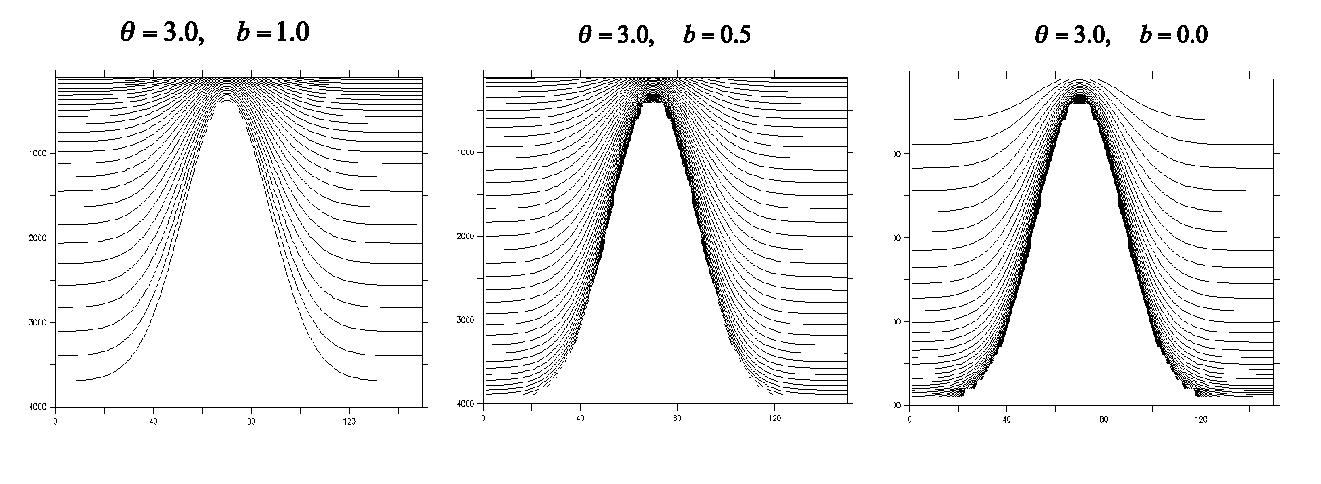
\includegraphics[width=0.66\textwidth]{DOMCFG_sco_function}
  \caption[DOMAINcfg: examples of the stretching function applied to a seamount]{
    Examples of the stretching function applied to a seamount;
    from left to right: surface, surface and bottom, and bottom intensified resolutions}
  \label{fig:DOMCFG_sco_function}
\end{figure}

where $H_c$ is the critical depth (\np{rn_hc}{rn\_hc}) at which the coordinate transitions from pure $\sigma$ to
the stretched coordinate, and $\theta$ (\np{rn_theta}{rn\_theta}) and $b$ (\np{rn_bb}{rn\_bb}) are the surface and
bottom control parameters such that $0 \leqslant \theta \leqslant 20$, and $0 \leqslant b \leqslant 1$.
$b$ has been designed to allow surface and/or bottom increase of the vertical resolution
(\autoref{fig:DOMCFG_sco_function}).

Another example has been provided at version 3.5 (\np{ln_s_SF12}{ln\_s\_SF12}) that allows a fixed surface resolution in
an analytical terrain-following stretching \citet{siddorn.furner_OM13}.
In this case the a stretching function $\gamma$ is defined such that:

\begin{equation}
  z = - \gamma h \quad \text{with} \quad 0 \leq \gamma \leq 1
  % \label{eq:DOMCFG_z}
\end{equation}

The function is defined with respect to $\sigma$, the unstretched terrain-following coordinate:

\begin{gather*}
  % \label{eq:DOMCFG_gamma_deriv}
  \gamma =   A \lt( \sigma   - \frac{1}{2} (\sigma^2     + f (\sigma)) \rt)
           + B \lt( \sigma^3 - f           (\sigma) \rt) + f (\sigma)       \\
  \intertext{Where:}
 \label{eq:DOMCFG_gamma}
  f(\sigma) = (\alpha + 2) \sigma^{\alpha + 1} - (\alpha + 1) \sigma^{\alpha + 2}
  \quad \text{and} \quad \sigma = \frac{k}{n - 1}
\end{gather*}

This gives an analytical stretching of $\sigma$ that is solvable in $A$ and $B$ as a function of
the user prescribed stretching parameter $\alpha$ (\np{rn_alpha}{rn\_alpha}) that stretches towards
the surface ($\alpha > 1.0$) or the bottom ($\alpha < 1.0$) and
user prescribed surface (\np{rn_zs}{rn\_zs}) and bottom depths.
The bottom cell depth in this example is given as a function of water depth:

\[
  % \label{eq:DOMCFG_zb}
  Z_b = h a + b
\]

where the namelist parameters \np{rn_zb_a}{rn\_zb\_a} and \np{rn_zb_b}{rn\_zb\_b} are $a$ and $b$ respectively.

\begin{figure}[!ht]
  \centering
  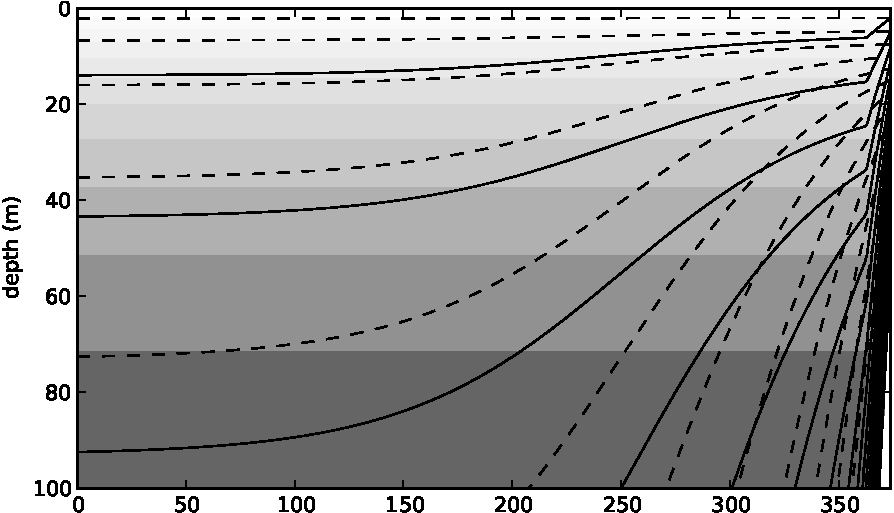
\includegraphics[width=0.66\textwidth]{DOMCFG_compare_coordinates_surface}
  \caption[DOMAINcfg: comparison of $s$- and $z$-coordinate]{
    A comparison of the \citet{song.haidvogel_JCP94} $S$-coordinate (solid lines),
    a 50 level $Z$-coordinate (contoured surfaces) and
    the \citet{siddorn.furner_OM13} $S$-coordinate (dashed lines) in the surface $100~m$ for
    a idealised bathymetry that goes from $50~m$ to $5500~m$ depth.
    For clarity every third coordinate surface is shown.}
  \label{fig:DOMCFG_fig_compare_coordinates_surface}
\end{figure}
 % >>>>>>>>>>>>>>>>>>>>>>>>>>>>

This gives a smooth analytical stretching in computational space that is constrained to
given specified surface and bottom grid cell thicknesses in real space.
This is not to be confused with the hybrid schemes that
superimpose geopotential coordinates on terrain following coordinates thus
creating a non-analytical vertical coordinate that
therefore may suffer from large gradients in the vertical resolutions.
This stretching is less straightforward to implement than the \citet{song.haidvogel_JCP94} stretching,
but has the advantage of resolving diurnal processes in deep water and has generally flatter slopes.

As with the \citet{song.haidvogel_JCP94} stretching the stretch is only applied at depths greater than
the critical depth $h_c$.
In this example two options are available in depths shallower than $h_c$,
with pure sigma being applied if the \np{ln_sigcrit}{ln\_sigcrit} is true and pure z-coordinates if it is false
(the z-coordinate being equal to the depths of the stretched coordinate at $h_c$).

Minimising the horizontal slope of the vertical coordinate is important in terrain-following systems as
large slopes lead to hydrostatic consistency.
A hydrostatic consistency parameter diagnostic following \citet{haney_JPO91} has been implemented,
and is output as part of the model mesh file at the start of the run.

%% =================================================================================================
\subsubsection[\zstar- or \sstar-coordinate (\forcode{ln_linssh})]{\zstar- or \sstar-coordinate (\protect\np{ln_linssh}{ln\_linssh})}
\label{subsec:DOMCFG_zgr_star}

This option is described in the Report by Levier \textit{et al.} (2007), available on the \NEMO\ web site.

\subinc{
\clearpage

%% Bibliography
\phantomsection
\addcontentsline{toc}{chapter}{Bibliography}
\lohead{Bibliography} \rehead{Bibliography}
\bibliography{../main/bibliography}

\clearpage

%% Indexes
\phantomsection
\addcontentsline{toc}{chapter}{Indexes}
\lohead{Indexes} \rehead{Indexes}
\printindex[blocks]
\printindex[keys]
\printindex[modules]
\printindex[parameters]
\printindex[subroutines]
}

\end{document}
